\subsubsection{Secondary structure}
%Translation initiation in prokaryotes begins after the ribosomal $30S$ subunit binds to the Shine-Dalgarno sequence and recognises the start codon. The larger subunit is then assembled to form a translation initiation complex, which moves along the transcript, decoding the codons to form a polypeptide chain. However, if this 
If the region around a translation initiation site forms a strong secondary structure, this leads to disruption of the formation of initiation complex, which inhibits translation (Figure \ref{fig:sec_str_rbs}) \cite{Kudla2009-tl, Espah_Borujeni2014-vy, Tuller2015-ts}. Recent studies show that the RNA structure stability of this region explains variation in protein expression better then codon usage \cite{Kudla2009-tl, Plotkin2011-ak, Cambray2018-kn} indicating that translation initiation is a rate limiting step for translation. Furthermore, secondary structure has been shown to change the functional half-life of mRNA and thus further influence protein expression \cite{mauger2019mrna}. Minimum free energy (MFE) of mRNA is widely used to measure the strength and stability of secondary structure. A way to find the MFE is to enumerate all possible structures of a given mRNA and then find the minimum. However, this is impractical because combinatorial explosion occurs quickly as the length of mRNA increases. Clever dynamic programming algorithms has made this problem tractable the details of which is described below.


\begin{figure}[htbp!]
\center
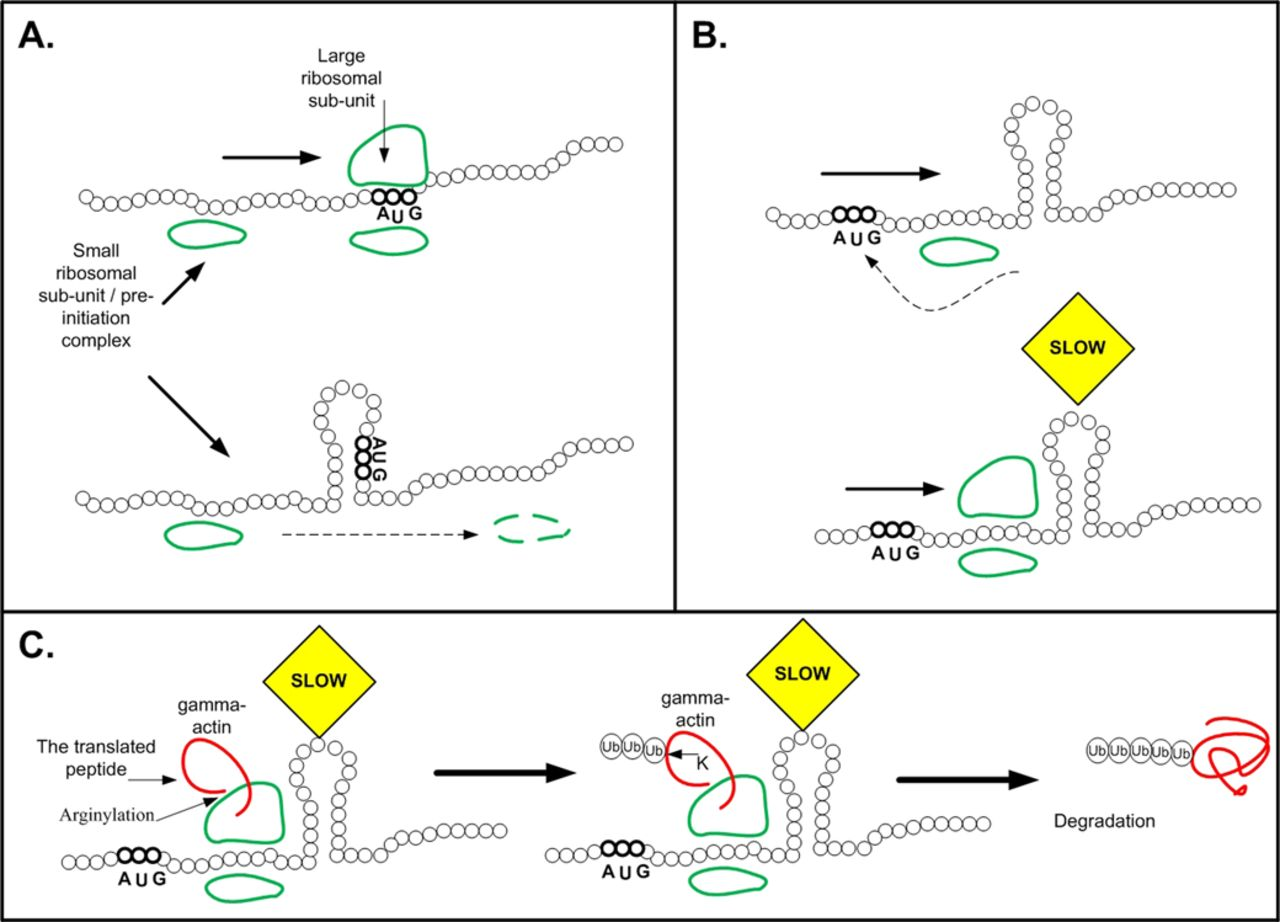
\includegraphics[width=1\textwidth]{chapters/Introduction/Figures/sec_str_rbs.jpg}
\caption[Secondary structure at the translation initiation site inhibits translation.]{\textbf{Secondary structure at the translation initiation site inhibits translation. (A) } The start codon AUG is recognised by the pre-initiation complex if the secondary structure is weak (top) but fails to do so in presence of a strong structure (bottom). \textbf{(B)} Presence of strong structure downstream of translation initiation site prevents the movement of pre-initiation complex (top) which could improve translation efficiency by improving ribosomal allocation (bottom). \textbf{(C)} Such downstream structures could influence post-translation modification by slowing down the ribosome. For example: lysin residues in arginylated gamma actin are exposed due to slow translation and undergo ubiquitination. Figure from Tuller and Zur, (2011) (Creative Commons license: CC BY ) }%the List of Figures because of the *}
\label{fig:sec_str_rbs}
\end{figure}



\paragraph{Computation of minimum free energy (MFE) and suboptimal structures}
Thermodynamically, an RNA structure with the lowest Gibb's free energy is the most stable. This energy is called minimum free energy. Thermodynamic ensembles usually follow the principle of locality, which says that interactions occur only between neighbouring particles. For example: In the Ising model of magnetism, spin interactions happen only between the nearest particles. Similarly, MFE is also calculated by using so called 'Turner parameters' \cite{turner2009nndb} in a nearest neighbouring model and a set of recursive equations called Zuker's algorithm \cite{zuker1981optimal}. However, the computed MFE is accurate only within $5-10\%$ and a large number of alternate RNA structures lie within $5-10\%$ of the predicted global minimum \cite{eddy2004rna}. This prompts us to calculate some other free energies for different suboptimal conformations that RNA may achieve in a near thermodynamic equilibrium. Furthermore, the suboptimal structures may not lie near the thermodynamic equilibrium. For example: Ding \textit{et al.} \cite{ding2005rna}  found that structures tend to form clusters in a Boltzmann ensemble. These are called centroid structures and the structures around the centroid may as well be regarded as suboptimal. 

There were some early attempts to compute suboptimal structures for example, by Zuker \cite{zuker1989finding} and Waterman \textit{et al.} \cite{waterman1985dynamic}. However, the backtracing procedure in their algorithms was not efficient enough to compute energies for longer RNA molecules. This problem was solved by McCaskill \cite{mccaskill1990equilibrium} by proposing an efficient algorithm to compute energy through a partition function which has the same time complexity as Zuker's algorithm for MFE $(\mathcal{O}(n^{3}))$.

\paragraph{Partition function and base pairing probabilities}
Consider a structure $s$ of an RNA molecule with free energy $E(s)$. In a thermodynamic ensemble of different structures at equilibrium, using the principle of maximum entropy, we see that the probability that the given RNA has the structure $s$ follows a Boltzmann distribution:

\begin{equation}
    p(s) \propto e^{-\beta E(s)}
\end{equation}

where $\beta$ is called 'thermodynamic beta' and equals $1/k_B T$, where $k_B$ is the Boltzmann's constant and $T$ is the absolute temperature (Subsection \ref{subsection:sim_anneal} Simulated annealing ). Since sum of probabilities over set of all structures $\Xi$, must be equal to unity, we have:

\begin{equation}
\begin{aligned}
    \sum_s p(s) &= \frac{1}{Z} \sum_{s\in\Xi} e^{-\beta E(s)}  = 1  \\
    Z &= \sum_{s\in\Xi} e^{-\beta E(s)} 
\end{aligned}
\label{eqn:part_func}
\end{equation}

The quantity $Z$, which plays a role of normalisation of probabilities, is called the \textit{canonical partition function}. Many thermodynamic parameters of interest can be derived from $Z$, for example, free energy $G$ in terms of $Z$ is given by:

\begin{equation}
\label{eqn:free_en}
    G = -\frac{1}{\beta} \ln(Z)
\end{equation}

The efficient dynamic programming to enumerate $Z$ was proposed by McCaskill \cite{mccaskill1990equilibrium} with time complexity of $\mathcal{O}(n^{3})$. This method is essentially a recursive decomposition of $Z$ similar to Zuker's algorithm only difference being the addition in Zuker's relation are now substituted by product because free energies are additive. If $E$ is the total free energy and $E_L$ are the energy contributions from various types of loops (hairpin, stacked pair, bulges, interior loops, multiloops) in a structure, then:

\begin{equation}
    E = \sum_L E_L
    \label{eqn:free_en_add}
\end{equation}

If we suppose the term $Q_{ij}^b$ accounts for all loops $L$ enclosed by $i,j$, we see that additivity of free energy (Equation \ref{eqn:free_en_add}) implies a multiplicative contribution to the partition function (\ref{eqn:part_func}) which gives the following recursive equation :

\begin{equation}
    Q_{ij}^b = \sum_L e^{-\beta E_L} \prod_{i<h<k<j} Q_{hk}^b
    \label{eqn:mcc_restr_part}
\end{equation}

Using this restricted partition function term for loop contributions, the total partition function between $i^{th}$ and $j^{th}$ nucleotides ($Q_{ij}$) can now be written as:

\begin{equation}
    Q_{ij} = Q_{i j-1} + \sum_{i \leq k <j} Q_{i k-1} Q_{kj}^b
    %where, by convention, Q_{i, i} = Q_{i, i-1} = 1.
    \label{eqn:mcc_full}
\end{equation}

The full partition function of RNA with $N$ nucleotides is given by $Z = Q_{1N}$. Equations \ref{eqn:mcc_restr_part} and \ref{eqn:mcc_full} are McCaskill's recursions for partition function. Once $Z$ is known, the probability of any structure $s$ with free energy $E(s)$ is given by:

\begin{equation}
\label{eqn:prob_part_func}
    p(s) = \frac{1}{Z} e^{-\beta E(s)}
\end{equation}

The computational approach outlined above is very generic and can be used for other specific cases. For example: if we want to know the probability that $[i^{th}, j^{th}]$ nucleotides are paired, then we can modify Equation \ref{eqn:part_func}, where partition function is found by simply summing Boltzmann's factor over all structures $\zeta \subseteq \Xi$ where $[i^{th}, j^{th}]$ nucleotides are paired:

\begin{equation}
    Z_p = \sum_{s\in\zeta} e^{-\beta E(s)}
\end{equation}

The base pairing probabilities are, given by equation \ref{eqn:prob_part_func} with an appropriately computed $Z$. % which is Z on the above equation.
